\documentclass[analysis_notes.tex]{subfiles}
\begin{document}
\section{Aula 25 - 29/05/2023}
\subsection{O que esperar?}
\begin{itemize}
	\item A integral de Riemann e de Riemann-Stieltjes;
	\item Integrais superiores e inferiores.
\end{itemize}
\subsection{Motiva\c cão}
\paragraph{Integrais de Riemann e Riemann-Stieltjes:}
Em matemática, a integral de Riemann é uma forma de definir a integral de uma
função sobre um intervalo. É definida como o limite dos somatórios de Riemann,
que são somas aproximadas calculadas a partir de valores da função em um
conjunto finito de pontos. A integral de Riemann usa partições do intervalo
de integração para calcular essas somas aproximadas.

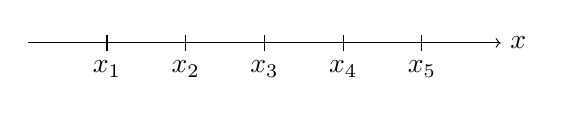
\begin{tikzpicture}
	\draw[->] (0,0) -- (6,0) node[right] {$x$};
	\foreach \x in {1,2,3,4,5}
	\draw (\x cm,3pt) -- (\x cm,-3pt) node[below] {$x_{\x}$};
\end{tikzpicture}

No gráfico acima, o intervalo de integração foi dividido em quatro subintervalos,
representados pelos pontos $x_1$, $x_2$, $x_3$, $x_4$ e $x_5$.
Cada subintervalo contribui para a soma de Riemann com um termo que é o
produto do valor da função em um ponto dentro do subintervalo pela largura do
subintervalo. À medida que a largura dos subintervalos diminui (ou seja, à
medida que aumentamos o número de pontos na partição), a soma de Riemann se
aproxima da área real sob a curva, que é a integral de Riemann da função.

A integral de Riemann-Stieltjes é uma generalização da integral de Riemann
que permite integrar funções com respeito a outras funções. Ao contrário da
integral de Riemann, que calcula a área sob uma curva em relação ao eixo x,
a integral de Riemann-Stieltjes calcula a "área" sob a curva de uma função em
relação a outra função.

\begin{tikzpicture}
	\draw[->] (-3,0) -- (4.2,0) node[right] {$x$};
	\draw[->] (0,-3) -- (0,4.2) node[above] {$y$};
	\draw[scale=0.5,domain=-3:3,smooth,variable=\x,blue] plot ({\x},{\x*\x});
	\draw[scale=0.5,domain=-3:3,smooth,variable=\x,red] plot ({\x},{\x*\x*\x});
\end{tikzpicture}

O gráfico acima mostra duas funções representadas em azul e vermelho.
A integral de Riemann da função azul seria a área sob a curva azul e acima
do eixo x. A integral de Riemann-Stieltjes da função vermelha com respeito à função
azul seria a "área" sob a curva vermelha e acima da curva azul. Podemos ter fun\c cões
que são Riemann-Stieltjes integrável, mas não Riemann integrável.

Considere a função de Dirichlet, que é definida como 1 para números racionais
e 0 para números irracionais. Esta função é notória por ser descontínua em todos
os pontos, o que a torna não integrável no sentido de Riemann.
No entanto, é possível mostrar que a função de Dirichlet é integrável no sentido
de Riemann-Stieltjes se a função que define a partição
(ou seja, a função em relação à qual estamos integrando) é de variação limitada.

\subsection{A Integral de Riemann}
A seguir, vamos representar, para \(a < b,\) a seguinte nota\c cão - \(\mathcal{B}([a,b], \mathbb{R})=\{f:[a,b]\rightarrow \mathbb{R}: f\text{ é limitada}\}.\)
\begin{def*}
	Dizemos que \(\mathcal{P}=\{x_{0}, x_{1}, \cdots, x_{n}\}\) é uma parti\c cão de \([a, b]\) se
	\[
		x_{0} = a < x_{1} < x_{2} < \cdots < x_{n-1} < x_{n} = b.
	\]
	Se \(\Delta x_{i}\coloneqq x_{i} - x_{i-1}, 1\leq i\leq n, ||P||\coloneqq \sup\{\Delta x_{i}: 1\leq i\leq n\}\) será chamada de
	malha da parti\c cão \(\mathcal{P}.\)

	Se \(f\in \mathcal{B}([a, b], \mathbb{R}), M_{i}=\sup_{x\in[x_{i-1},x_{i}]}f(x), m_{i}=\inf_{x\in[x_{i-1}, x_{i}]f(x)}\) e
	chamamos de soma superior e inferior da fun\c cão f relativas à \(\mathcal{P},\) as somas
	\[
		U(\mathcal{P}, f) = \sum\limits_{i=1}^{n}M_{i}\Delta x_{i},\quad L(\mathcal{P}, f)=\sum\limits_{i=1}^{n}m_{i}\Delta x_{i}.
	\]
\end{def*}
Note que
\begin{itemize}
	\item \(\sum\limits_{i=1}^{n}\Delta x_{i} = b-a\);
	\item \(L(\mathcal{P}, f)\leq U(\mathcal{P}, f)\) pois \(m_{i}\leq M_{i}, 1\leq i\leq n\);
	\item \(m=\inf_{x\in[a, b]}f(x)\) e \(M=\sup_{x\in[a, b]}f(x), m\leq m_{i}\leq M_{i}\leq M, 1\leq i\leq n\);
	\item \(m(b-a)\leq L(\mathcal{P}, f) = \sum\limits_{i=1}^{n}m_{i}\Delta x_{i}\leq \sum\limits_{i=1}^{n} M_{i}\Delta x_{i}=U(\mathcal{P}, f)\leq M(b-a)\)
	\item Os conjuntos \(\{U(\mathcal{P}, f): \mathcal{P}\in \mathfrak{P}_{[a, b]}\}\) e
	      \(\{L(\mathcal{P}, f): \mathcal{P}\in \mathfrak{P}_{[a, b]}\}\) são limitados inferiormente e superiormente, respecitvamente,
	      em que \(\mathfrak{P}_{[a, b]} = \{\mathcal{P}: \mathcal{P}\text{ é parti\c cão de }[a, b]\}\).
\end{itemize}
\begin{def*}
	Definimos a integral superior de Riemann de f em \([a, b]\) por
	\[
		\overline{\int_{a}^{b}}f(x)dx = \inf_{\mathcal{P}\in \mathfrak{P}}U(\mathcal{P}, f)
	\]
	e a integral inferior de Riemann de f em \([a, b]\) por
	\[
		\underline{\int_{a}^{b}}f(x)dx = \sup_{\mathcal{P}\in \mathfrak{P}}L(\mathcal{P}, f).
	\]
	Caso \(\overline{\int_{a}^{b}}f(x)dx = \underline{\int_{a}^{b}}f(x)dx\), diremos que f é Riemann
	integrável em \([a, b]\). O valor comum acima é chamado integral de Riemann de f em
	\([a, b]\), sendo denotado por \(\int_{a}^{b}f(x)dx\). Além disso,
	\(\mathfrak{R}([a, b]) = \{f\in \mathfrak{B}([a, b], \mathbb{R}): f\text{ é Riemann integrável em }[a, b]\}.\square\)
\end{def*}
\begin{example}
	Nem toda fun\c cão limitada é Riemann integrável. De fato, seja \(f:[0, 1]\rightarrow \mathbb{R}\) dada por
	\[
		f(x) \coloneqq  \left\{\begin{array}{ll}
			0,\quad x\in \mathbb{Q}\cap{[0, 1]} \\
			1,\quad x\in \mathbb{I}\cap{[0, 1]}.
		\end{array}\right.
	\]
	Vamos mostrar que, apesar de limitada, f não é Riemann integrável em \([0, 1].\)

	De fato, se \(\mathcal{P} = \{0 = x_{0}, x_{1}, \cdots, x_{n} = 1\}\in \mathfrak{P}_{[0, 1]},\) como \(M_{i}=\sup_{x\in[x_{i-1}, x_{i}]} f(x) = 1\)
	e \(m_{i} = \inf_{x\in[x_{i-1}, x_{i}]}f(x) = 0,\)
	\begin{align*}
		 & U(\mathcal{P}, f) = \sum\limits_{i=1}^{n}M_{i}\Delta x_{i} = \sum\limits_{i=1}^{n}\Delta x_{i} =1,   \\
		 & L(\mathcal{P}, f) = \sum\limits_{i=1}^{n}m_{i}\Delta x_{i} = \sum\limits_{i=1}^{n}0\Delta x_{i} = 0.
	\end{align*}
	Sendo assim,
	\[
		\overline{\int_{0}^{1}}f(x)dx = 1\neq \underline{\int_{0}^{1}}f(x)dx = 0.
	\]
	Portanto, f não é Riemann integrável em \([0, 1].\)
\end{example}
\subsection{A Integral de Riemann-Stieltjes}
Para introduzir a integral de Riemann-Stieltjes, seja \(\alpha :[a, b]\rightarrow \mathbb{R}\) não-crescente. Claramente, \(\alpha \) é limitada em \([a, b]\).
Dada \(\mathcal{P}=\{x_{0}, x_{1}, \cdots, x_{n}\}\in \mathfrak{P}_{[a, b]}\) para \(1\leq i\leq n\), seja
\[
	\Delta \alpha_{i} = \alpha (x_{i}) - \alpha (x_{i-1})\geq 0,\quad 1\leq i\leq n.
\]
Além disso, dada \(f\in \mathfrak{B}([a, b], \mathbb{R}),\) defina
\begin{align*}
	 & U(\mathcal{P}, f, \alpha ) = \sum\limits_{i=1}^{n}M_{i}\Delta \alpha_{i}, \\
	 & L(\mathcal{P}, f, \alpha ) = \sum\limits_{i=1}^{n}m_{i}\Delta \alpha_{i},
\end{align*}
sendo \(M_{i} = \sup_{x\in[x_{i-1}, x_{i}]}f(x), m_{i} = \inf_{x\in[x_{i-1}, x_{i}]}f(x),\) como antes.
Note que
\[
	\sum\limits_{i=1}^{n}\Delta \alpha_{i} = \alpha (b) - \alpha (a)
\]
e
\begin{align*}
	 & L(\mathcal{P}, f, \alpha ) = \sum\limits_{i=1}^{n}m_{i}\Delta \alpha_{i}\leq \sum\limits_{i=1}^{n}M_{i}\Delta \alpha_{i} = U(\mathcal{P}, f, \alpha ) \\
	 & m[\alpha (b) - \alpha (a)] = \sum\limits_{i=1}^{n}m\Delta \alpha_{i}\leq \sum\limits_{i=1}^{n}M_{i}\Delta \alpha_{i} = U(\mathcal{P}, f, \alpha )     \\
	 & L(\mathcal{P}, f, \alpha ) = \sum\limits_{i=1}^{n}m_{i}\Delta \alpha_{i}\leq M \sum\limits_{i=1}^{n}\Delta \alpha_{i} = M[\alpha (b)-\alpha (a)],
\end{align*}
em que \(m = \inf_{x\in[a,b]}f(x)\) e \(M=\sup_{x\in[a, b]}f(x).\) Disto segue que os conjuntos
\[
	\{L(\mathcal{P}, f, \alpha ): \mathcal{P}\in \mathfrak{P}_{[a, b]}\}\quad\text{ e } \{U(\mathcal{P}, f, \alpha ): \mathcal{P}\in \mathfrak{P}_{[a, b]}\}
\]
são, respectivamente, limitado superiormente e inferiormente em \(\mathbb{R}.\) Definimos a integral superior
e inferior de Riemann-Stieltjes para uma fun\c cão f em \([a, b]\) relativas à \(\alpha \) analogamente às de Riemann :
\[
	\overline{\int_{a}^{b}}f d\alpha =\inf_{P\in \mathfrak{P}}U(\mathcal{P}, f, \alpha ) \text{ e } \underline{\int_{a}^{b}}f d\alpha =\sup_{\mathcal{P}\in \mathfrak{P}}L(\mathcal{P}, f, \alpha ).
\]
\begin{def*}
	A fun\c cão f é Riemann-Stieltjes integrável em \([a, b]\) relativamente a \(\alpha \) se
	\[
		\overline{\int_{a}^{b}}f d\alpha  = \underline{\int_{a}^{b}}fd\alpha .
	\]
	O valor acima é chamado integral de Riemann-Stieltjes de f em \([a, b]\) relativamente à fun\c cão \(\alpha \), sendo denotado por
	\[
		\int_{a}^{b} f d\alpha \text{ ou } \int_{a}^{b} f(x) d\alpha (x). \square
	\]
\end{def*}
Denote por \(\mathfrak{R}(\alpha , [a, b]) = \{f\in \mathfrak{B}([a, b], \mathbb{R}): f\text{ é Riemann-Stieltjes integrável em }[a, b],\text{ relativamente a }\alpha \}\).

Se \(\alpha :[a, b]\rightarrow \mathbb{R}\) é dada por \(\alpha (x) = x, x\in[a, b]\), a integral de Riemann-Stieltjes, relativamente a \(\alpha \), coincide
com a integral de Riemann, ou seja,
\[
	\int_{a}^{b}f d\alpha = \int_{a}^{b}f(x)dx
\]
pois, neste caso, \(\delta x_{i}=\alpha (x_{i}) - \alpha (x_{i=1}) = x_{i} - x_{i-1} = \Delta x_{i}, 1\leq i\leq n\).

Observe que \(\alpha :[a, b]\rightarrow \mathbb{R}\) só precisa ser não-decrescente em \([a, b],\) para
podermos definir a integral de Riemann-Stieltjes de fun\c cões \(f\in \mathfrak{B}([a, b], \mathbb{R})\) relativamente a \(\alpha .\)

Vamos supor, adiante, que \(\alpha (b) > \alpha (a).\) Caso contrário, a integral de Riemann-Stieltjes de f
relativamente a \(\alpha \) seria nula para toda \(f\in \mathfrak{B}([a, b], \mathbb{R})\).
\begin{def*}
	Sejam \(\mathcal{P}, \mathcal{P}^{*}\in \mathfrak{P}_{[a, b]}\). Dizemos que a parti\c cão \(\mathcal{P}^{*}\) é um
	refinamento da parti\c cão \(\mathcal{P}\) se
	\[
		\mathcal{P}\subseteq{\mathcal{P}^{*},}
	\]
	ou seja, todo ponto de \(\mathcal{P}\) é um ponto de \(\mathcal{P}^{*}. \square\)
\end{def*}
Sejam \(\mathcal{P}_{1}, \mathcal{P}_{2}\in \mathfrak{P}_{[a, b]}.\) Definimos
\[
	\mathcal{P}^{*} = \mathcal{P}_{1}\cup \mathcal{P}_{2}.
\]
Então, \(\mathcal{P}\in \mathfrak{P}_{[a, b]}\) e \(\mathcal{P}^{*}\) é um refinamento comum
a \(\mathcal{P}_{1}\) e a \(\mathcal{P}_{2}.\)
\begin{prop*}
	Sejam \(\mathcal{P}, \mathcal{P}^{*}\in \mathfrak{P}_{[a, b]}\) com \(\mathcal{P}^{*}\supseteq{\mathcal{P}.}\) Então,
	\begin{align*}
		 & L(\mathcal{P}, f, \alpha )\leq L(\mathcal{P}^{*}, f, \alpha )  \\
		 & U(\mathcal{P}^{*}, f, \alpha )\leq U(\mathcal{P}, f, \alpha ).
	\end{align*}
\end{prop*}
\begin{proof*}
	Se \(\mathcal{P}^{*} = \mathcal{P}\), não há o que fazer. Se \(\mathcal{P}\subsetneq{P}^{*},\) seja \(x^{*}\in \mathcal{P}^{*}\backslash \mathcal{P}.\) Considere,
	inicialmente, o caso
	\[
		\mathcal{P}^{*} = \mathcal{P}\cup\{x^{*}\}.
	\]
	Logo, se \(\mathcal{P}\) tem n elementos, \(\mathcal{P}^{*}\) tem n+1 elementos e
	\begin{align*}
		 & \mathcal{P} = \{a = x_{0}, x_{1}, \cdots, x_{i_{0}-1}, x_{i_{0}}, \cdots, x_{n} = b\},                              \\
		 & \mathcal{P}^{*} = \{a = x_{0}^{*}, x_{1}^{*}, \cdots, x_{i_{0}-1}^{*}, x, x_{i_{0}+1}^{*}, \cdots, x_{n}^{*} = b\}, \\
		 & =\{a = x_{0}^{*}, x_{1}^{*}, \cdots, x_{i_{0}-1}^{*}, x_{i_{0}}^{*}, \cdots, x_{n+1}^{*} = b\},                     \\
	\end{align*}
	se \(m_{i} = \inf_{x\in[x_{i-1}, x_{i}]}f(x), 1\leq i\leq n\) e \(m_{j}^{*} = \inf_{x\in[x_{j-1}^{*}, x_{j}^{*}}f(x), 1\leq j\leq n+1,\) colocamos
	\(\Delta \alpha_{i} = \alpha (x_{i}) - \alpha (x_{i-1}), 1\leq i\leq n\) e \(\Delta \alpha_{j}^{*} = \alpha (x_{j}^{*}) - \alpha (x_{j-1}^{*}), 1\leq j\leq n+1.\)

	Assim,
	\begin{align*}
		L(\mathcal{P}^{*}, f, \alpha ) - L(\mathcal{P}, f, \alpha ) & = \sum\limits_{j=1}^{n+1}m_{j}^{*}\Delta \alpha_{j}^{*} - \sum\limits_{i=1}^{n}m_{i}\Delta \alpha_{i}                                                                        \\
		                                                            & = m_{i_{0}}^{*}\Delta \alpha_{i_{0}}^{*} + m_{i_{0}+1}^{*}\Delta \alpha _{i_{0}+1}^{*} - m_{i_{0}}\Delta \alpha _{i_{0}}                                                     \\
		                                                            & = m_{i_{0}}^{*}\Delta \alpha_{i_{0}}^{*} + m_{i_{0}+1}^{*}\Delta \alpha _{i_{0}+1}^{*} - m_{i_{0}}[\alpha (x_{i_{0}}) - \alpha (x^{*})+\alpha (x^{*}) - \alpha (x_{i_{0}-1}) \\
		                                                            & = [m_{i_{0}}^{*} - m_{i_{0}}][\alpha (x^{*}) - \alpha (x_{i_{0}-1})] + [m_{i_{0}+1}^{*} - m_{i_{0}}][\alpha (x_{i_{0}}) - \alpha (x^{*}]\geq 0.
	\end{align*}
	Em outras palavras,
	\[
		L(\mathcal{P}^{*}, f, \alpha ) - L(\mathcal{P}, f, \alpha )\geq 0.
	\]
	O caso geral segue por indu\c cão. A desigualdade para a soma superior é obtida de maneira análoga (Exercício). \(\square\)
\end{proof*}
\begin{theorem*}
	Seja \(f:[a, b]\rightarrow \mathbb{R}\) limitada em \([a, b]\). Então,
	\[
		\underline{\int_{a}^{b}} f d\alpha\leq \overline{\int_{a}^{b}}f d\alpha .
	\]
\end{theorem*}
\begin{proof*}
	Do resultado anterior, se \(\mathcal{P}_{1}, \mathcal{P}_{2}\in \mathfrak{P}_{[a, b]}\) e \(\mathcal{P}^{*} = \mathcal{P}_{1}\cup \mathcal{P}_{2}\),
	\[
		L(\mathcal{P}_{1}, f, \alpha )\leq L(\mathcal{P}^{*}, f, \alpha )\leq U(\mathcal{P}^{*}, f, \alpha )\leq U(P_{2}, f, \alpha ).
	\]
	Portanto,
	\[
		\underline{\int_{a}^{b}}f d\alpha =\sup_{\mathcal{P_{1}}\in \mathfrak{P}}\leq \inf_{\mathcal{P}_{2}\in \mathfrak{P}} U(\mathcal{P}_{2}, f, \alpha ) = \overline{\int_{a}^{b}}f d\alpha .\text{ \qedsymbol}
	\]
\end{proof*}
\begin{crl*}
	Seja \(f:[a, b]\rightarrow \mathbb{R}\) uma fun\c cão limitada em \([a, b].\) Então, \(f\in \mathfrak{R}(\alpha , [a, b])\) se, e somente se,
	dado \(\varepsilon >0\), existe uma parti\c cão \(P\in \mathfrak{P}\) tal que
	\[
		0\leq U(\mathcal{P}, f, \alpha ) - L(\mathcal{P}, f, \alpha ) <\varepsilon .
	\]
\end{crl*}
\begin{proof*}
	Note que, dado \(\varepsilon  >0\), se \(\mathcal{P}\in \mathfrak{P}\) é tal que a desigualdade acima está satisfeita,
	\begin{align*}
		 & L(\mathcal{P}, f, \alpha )\leq \sup_{\mathcal{P}'\in \mathfrak{P}}L(\mathcal{P}', f, \alpha ) = \underline{\int_{a}^{b}}f d\alpha     \\
		 & \leq \overline{\int_{a}^{b}}f d\alpha = \inf_{\mathcal{P}'\in \mathfrak{P}}U(\mathcal{P}', f, \alpha )\leq U(\mathcal{P}, f, \alpha )
	\end{align*}
	e
	\[
		0\leq \overline{\int_{a}^{b}}f d\alpha  - \underline{\int_{a}^{b}}f d\alpha\leq U(\mathcal{P}, f, \alpha ) - L(\mathcal{P}, f,\alpha ) <\varepsilon .
	\]
	Logo, \(f\in \mathfrak{R}(\alpha, [a,b])\).

	Por outro lado, se \(f\in \mathfrak{R}(\alpha , [a,b]),\)
	\[
		\inf_{P\in \mathfrak{P}}U(\mathcal{P}, f, \alpha ) = \sup_{P\in \mathfrak{P}}L(\mathcal{P}, f, \alpha ).
	\]
	Assim, dado \(\varepsilon >0\), existem parti\c cões \(\mathcal{P}_{1}, \mathcal{P}_{2}\in \mathfrak{P}\) tais que
	\[
		U(\mathcal{P}, f, \alpha )\leq U(\mathcal{P}_{2}, f, \alpha ) < \overline{\int_{a}^{b}}f d\alpha +\frac{\varepsilon }{2} = \int_{a}^{b} f d\alpha  + \frac{\varepsilon }{2},
	\]
	e,
	\[
		L(\mathcal{P}, f, \alpha )\geq L(\mathcal{P}_{1}, f, \alpha ) > \underline{\int_{a}^{b}} f d\alpha - \frac{\varepsilon }{2} = \int_{a}^{b}f d\alpha - \frac{\varepsilon }{2},
	\]
	em que \(\mathcal{P} = \mathcal{P}_{1}\cup \mathcal{P}_{2}.\) Portanto, \(0\leq U(\mathcal{P}, f, \alpha ) - L(\mathcal{P}, f, \alpha ) < \varepsilon .\) \qedsymbol
\end{proof*}
\begin{theorem*}
	Seja \(f:[a, b]\rightarrow \mathbb{R}\) é limitada e \(\varepsilon  > 0\) dado.
	\begin{itemize}
		\item[1)] Se existe parti\c cão P tal que \(0\leq U(\mathcal{P}, f, \alpha ) - L(\mathcal{P}, f, \alpha )  < \varepsilon \), então
		      \(0\leq U(\mathcal{P}^{*}, f, \alpha ) - L(\mathcal{P}^{*}, f, \alpha ) < \varepsilon \), para todo refinamento \(\mathcal{P}^{*}\) de \(\mathcal{P}.\)
		\item[2)] Se existe \(P = \{a = x_{0}, x_{1}, \cdots, x_{n} = b\}\) tal que \(0\leq U(\mathcal{P}, f, \alpha ) - L(\mathcal{P}, f, \alpha ) < \varepsilon \) e, para
		      cada \(1\leq i\leq n\), dados \(s_{i}, t_{i}\in [x_{i-1}, x_{i}], \) então
		      \[
			      \sum\limits_{i=1}^{n}|f(s_{i}) - f(t_{i})|\Delta \alpha_{i} < \varepsilon
		      \]
		      e, se \(f\in \mathfrak{R}(\alpha , [a, b]),\)
		      \[
			      \biggl|\sum\limits_{i=1}^{n}f(t_{i})\Delta \alpha_{i} - \int_{a}^{b}f d\alpha\biggr| < \varepsilon .
		      \]
	\end{itemize}
\end{theorem*}
\begin{proof*}
	1) Seja P uma parti\c cão tal que \(0\leq U(\mathcal{P}, f, \alpha ) - L(\mathcal{P}, f, \alpha ) < \varepsilon \) e
	\(\mathcal{P}^{*}\) um refinamento de \(\mathcal{P}.\) O resultado segue de
	\[
		L(\mathcal{P}, f, \alpha )\leq L(\mathcal{P}^{*}, f, \alpha )\leq U(\mathcal{P}^{*}, f, \alpha )\leq U(\mathcal{P}, f, \alpha ).
	\]

	2) Sabemos que, para cada \(i\in\{1, 2, \cdots, n\}\), se \(s_{i}, t_{i}\in [x_{i-1}, x_{i}]\), então
	\(f(s_{i}), f(t_{i})\in[m_{i}, M_{i}]\) e \(|f(s_{i})-f(t_{i})|\leq M_{i} - m_{i},\) em que
	\(m_{i} = \inf_{x\in[x_{i-1}, x_{i}]}f(x)\) e \(M_{i}=\sup_{x\in[x_{i-1}, x_{i}]}f(x)\). Portanto,
	\[
		\sum\limits_{i=1}^{n}|f(s_{i})-f(t_{i})|\Delta \alpha_{i}\leq \sum\limits_{i=1}^{n}(M_{i}-m_{i})\Delta \alpha_{i} = U(\mathcal{P}, f, \alpha )-L(\mathcal{P}, f, \alpha ) <\varepsilon
	\]
	e o resultado segue. Agora, se \(f\in \mathfrak{R}(\alpha , [a, b])\), dado \(\varepsilon >0\), existe uma
	parti\c cão P de \([a, b]\) tal que
	\[
		L(\mathcal{P}, f, \alpha )\leq \int_{a}^{b}f d\alpha \leq U(\mathcal{P}, f, \alpha ) < L(\mathcal{P}, f, \alpha ) + \varepsilon .
	\]
	Escolhendo \(t_{i}\in[x_{i-1}, x_{i}], f(t_{i})\in[m_{i}, M_{i}],\)
	\begin{align*}
		L(\mathcal{P}, f, \alpha ) & = \sum\limits_{i=1}^{n}m_{i}\Delta \alpha_{i}\leq \sum\limits_{i=1}^{n}f(t_{i})\Delta \alpha_{i}                         \\
		                           & \leq \sum\limits_{i=1}^{n}M_{i}\Delta\alpha_{i} = U(\mathcal{P}, f, \alpha ) < L(\mathcal{P}, f, \alpha ) + \varepsilon.
	\end{align*}
	Portanto, o resultado está provado. \qedsymbol
\end{proof*}
\end{document}
